\subsection{Fator $\gamma$ do ar: Método de Rüchardt}

Como introduzido no experimento anterior, o fator $\gamma$ é uma propriedade intrínseca dos gases, muito interessante e importante se ter conhecimento. Para isso, utilizaremos agora uma outra forma de determiná-lo.

Nesse experimento, elaborado pelo físico alemão Eduard Rüchardt, utilizaremos o mesmo princípio do anterior: pressurizaremos um recipiente com uma bomba manual e liberaremos rapidamente esse ar para realizar aquele processo termodinâmico como visto na Figura \ref{fig:processo-grafico}.

A diferença aqui virá do fato que temos na montagem experimental uma bolinha que se encontra em equilíbrio com a pressão interna e a atmosférica, pois ela cria uma vedação com o tudo alongado. Isso quer dizer que qualquer variação de pressão dentro do recipiente (provocada por um processo de compressão e rápida descompressão, por exemplo) ocasionará um movimento nela.

\begin{figure}[H]
  \centering
  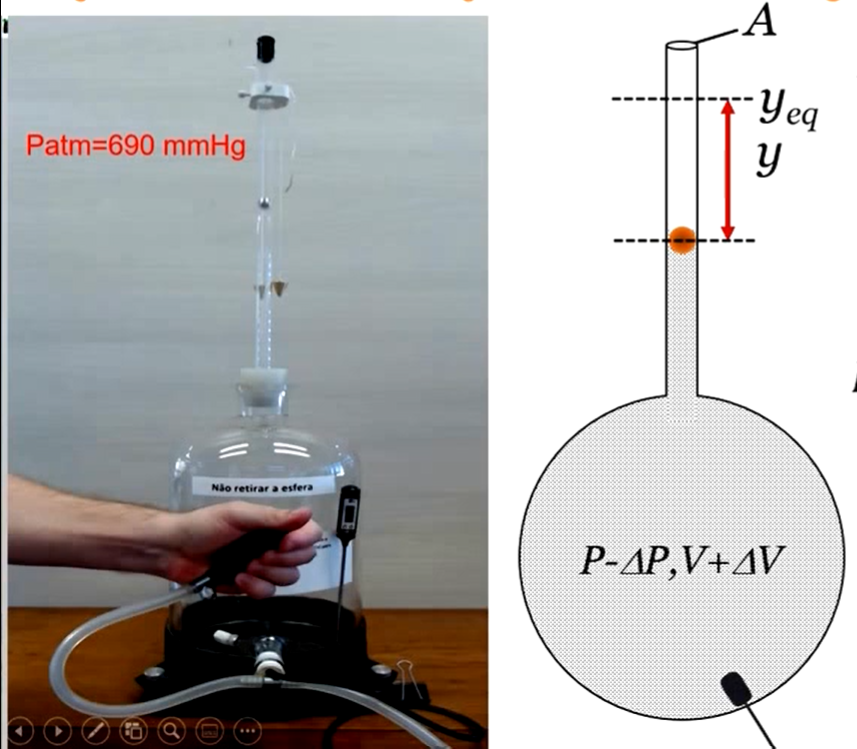
\includegraphics[scale=0.7]{images/montagem-ruchardt.png}
  \caption{Montagem experimental e diagrama do Método de Rüchardt}
\end{figure}

Desenvolvendo as equações de equilíbrio de forças presentes nesse experimento que foram vistas na videoaula dessa prática, chegamos na seguinte relação:

\[ \ddot{y} + \left( \frac{\gamma P A^2}{m V} \right) y = 0 \]

Essa equação é característica de um movimento harmônico, ou seja, a bolinha oscilará (amortecidamente, já que vivemos num mundo não ideal onde existe atrito e resistência do ar) no final do processo. Sendo assim, medindo o período de oscilação (T) nós podemos encontrar o desejado $\gamma$ do ar atmosférico.\\

Então, utilizaremos um microfone interno para captar as variações periódicas de pressão, e com um software de análise sonora podemos obter o período mencionado. Com esse valor e as características dos equipamentos e ambiente em mãos, como a massa da boinha (m), área do tubo (A), volume do recipiente (V) e a pressão atmosférica (P), podemos falar que a característica $\gamma$ do ar pode ser definida como:

\[ N = m \cdot V \]
\[ D = P \cdot A^2 \cdot T^2 \]
\[ \therefore \gamma = 4\pi^2 \cdot \frac{N}{D} \]

E a sua incerteza \textbf{VERIFICAR ISSO AQUI PQ PODE N ESTAR CERTO}:

\begin{table}[H]
    \centering
    \begin{tabular}{ c|c  }
         $\delta N = \delta m \cdot V + m \cdot \delta V$ &
         $\delta a = 2 \cdot A \cdot \delta A$\\
         \hline \\
         $\delta D = P \cdot (A \cdot \delta t + \delta a \cdot T)$ &
         $\delta t = 2 \cdot T \cdot \delta T$\\
    \end{tabular}
\end{table}

\[ \therefore \delta \gamma = 4\pi^2 \cdot \frac{N \cdot \delta D + \delta N \cdot D}{D^2}\]

*as fórmulas foram quebradas para facilitar nos cálculos
